\begin{figure}[H]
  \caption{Three tiers architecture of the system}
  \label{3tiers}
  \centering
  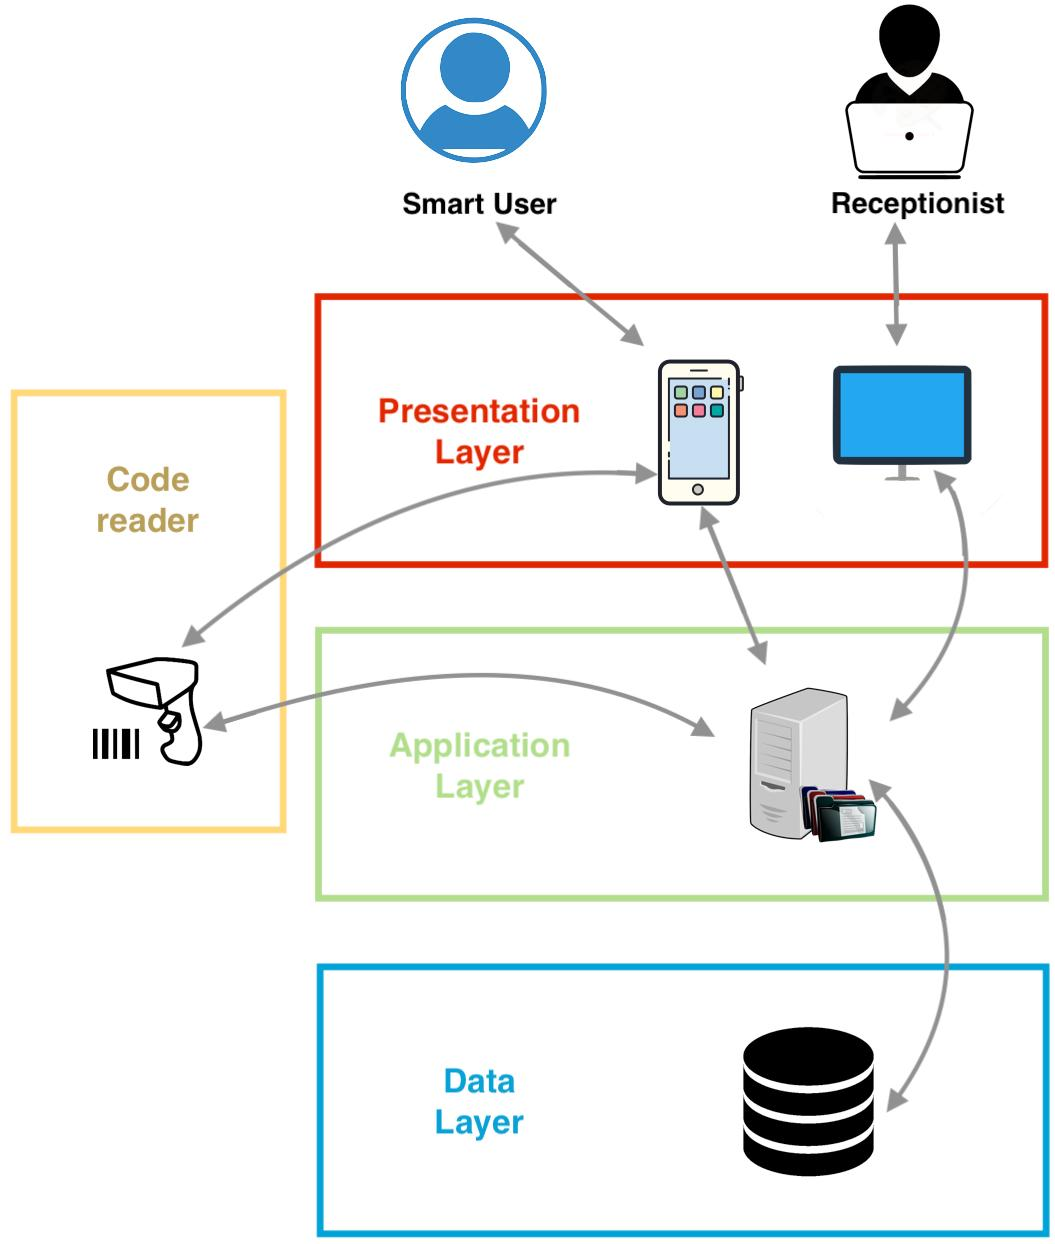
\includegraphics[scale=0.25]{diagrams/3_tiers.jpeg}

\end{figure}


\section{Overview: High-level components and their interaction}
The system is organized following the three tiers architecture. This aims to decouple logical layers in order to gurantee an horizontal scalability and an high fault tolerance.
Graphically it's shown in the figure~\ref{3tiers}.
\par

\textbf{Presentation layer}. It's the front-end layer which consists of the user interface. We have two types of user interface, depending on his functionality: 
\begin{itemize}
\item \textbf{CLup}: It's the mobile application used by users who have a smartphone. They can manage their booking by themselves;
\item \textbf{CLup Operator}: It's the desktop application used by receptionists that act as an intermediary to manage booking of users that have only a mobilephone.
\end{itemize}

\textbf{Application layer}. It deals with the model of the system, by containing the business logic of the application. In our system it consists in a remote server to which mobile and desktop applications have to connect due to manage any bookings.

\textbf{Data layer}. It's composed by a data storage system. It includes: 

\begin{itemize}
\item User sensitive data asked during the registration process;
\item Information about user's grocery shopping;
\end{itemize}



\section{Component view}


\begin{figure}[H]
  \label{fig:highlevel}
  \centering
  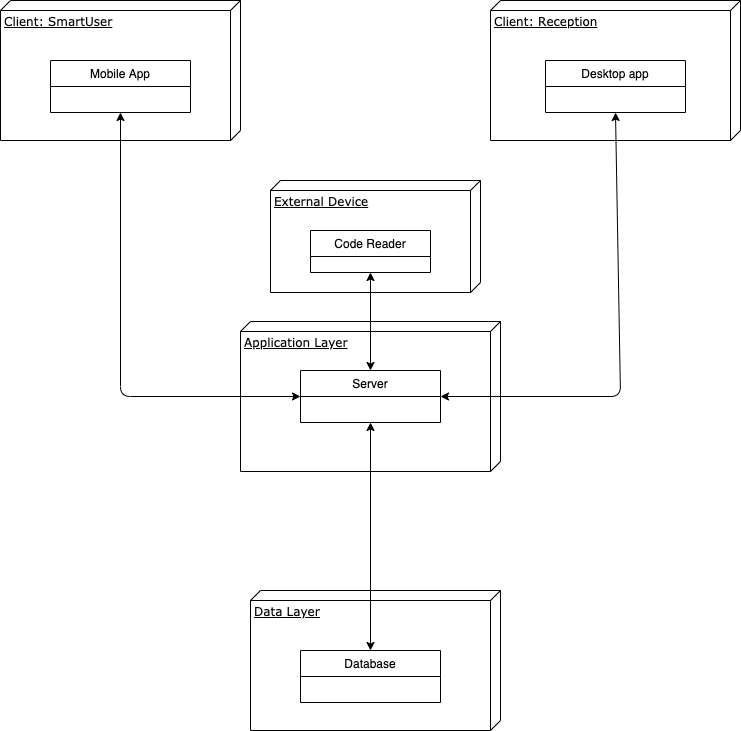
\includegraphics[scale=0.25]{diagrams/h_level.png}
  \caption{High-Level component diagram}
\end{figure}


In this section we describe the architecure with respect to its components and how they are wired together to form our system. 
Indeed, communication between Server and Clients is ensured by appropriate components which are called \textbf{Network Manager}. 
By an high-level point of view (figure~\ref{fig:highlevel}) the main subsysystems correspond almost to the 3 layers in the 3 tiers architecture, with the addition of the \textbf{Market's subsystem}. The last one includes the \textbf{QRCode reader}, which has different functionality:
\begin{itemize}
\item It checks if QRCode at the entrance is valid. If it's valid it will submit it. In addition a manual insertion of the QRCode is provided, due to allows Mobile Users to insert his code sent by SMS;
\item It controls the \textbf{Shop door}. If a QRCode is submitted, the reader allows users to enter by opening it;
\end{itemize}

It follows a detailed description of the other significant components.

\subsection{Application layer}
It's the core of our system. It's composed by:
\begin{itemize}
\item \textbf{CLup}: In our model this component acts as a controller. It deals with the stochastic time estimations to control the flux of users inside and outside the market. Moreover this component [...] 
In order to do that, it's also linked to the DB which provides data that are going to be processed and analysed;
\item \textbf{Auth User and Auth Reception}: these components grants respectively the access of users and receptionist by verifying their credential. In particular they are also accountable for users' registration;
\item \textbf{Visit Schedule and Reservation Queue}: they manage respectevely Visit and Reservation requests of Users and Receptionists. In addition They provides QRCodes to the clients;
\item \textbf{Notification Manager}: it's the component necessary to notify users about their turn in the queue;
\end{itemize}


\subsection{Client's layers: CLup and CLup Operator}
Each one of them is composed by components in a similar way, even if they have different functionalities.
Both they've got, as we can see in the figure~\ref{component_diagram}:
\begin{itemize} 
\item \textbf{GUI component}: it provides the graphical interface in which User and Receptionist can interact with the system;
\item \textbf{Network Manager}: it's used to interact with the application server by sending or receiving informations; 
\end{itemize}


In addition CLup is composed by a \textbf{Request Handler} which exposes methods to User to handle his booking. Then, it interract with the Network Manager to send request to the Server. 

Instead, CLup Operator has the \textbf{Booking Manager}, which is a similar component to the previous one but with more functionalities. In particular it handles any booking of mobile users and their sensitive information. So it's allowed by application server to query all users' sensitive data with higher privileges than CLup.




\begin{figure}[h]
  \label{component_diagram}
  \centering
  \makebox[\linewidth]{
  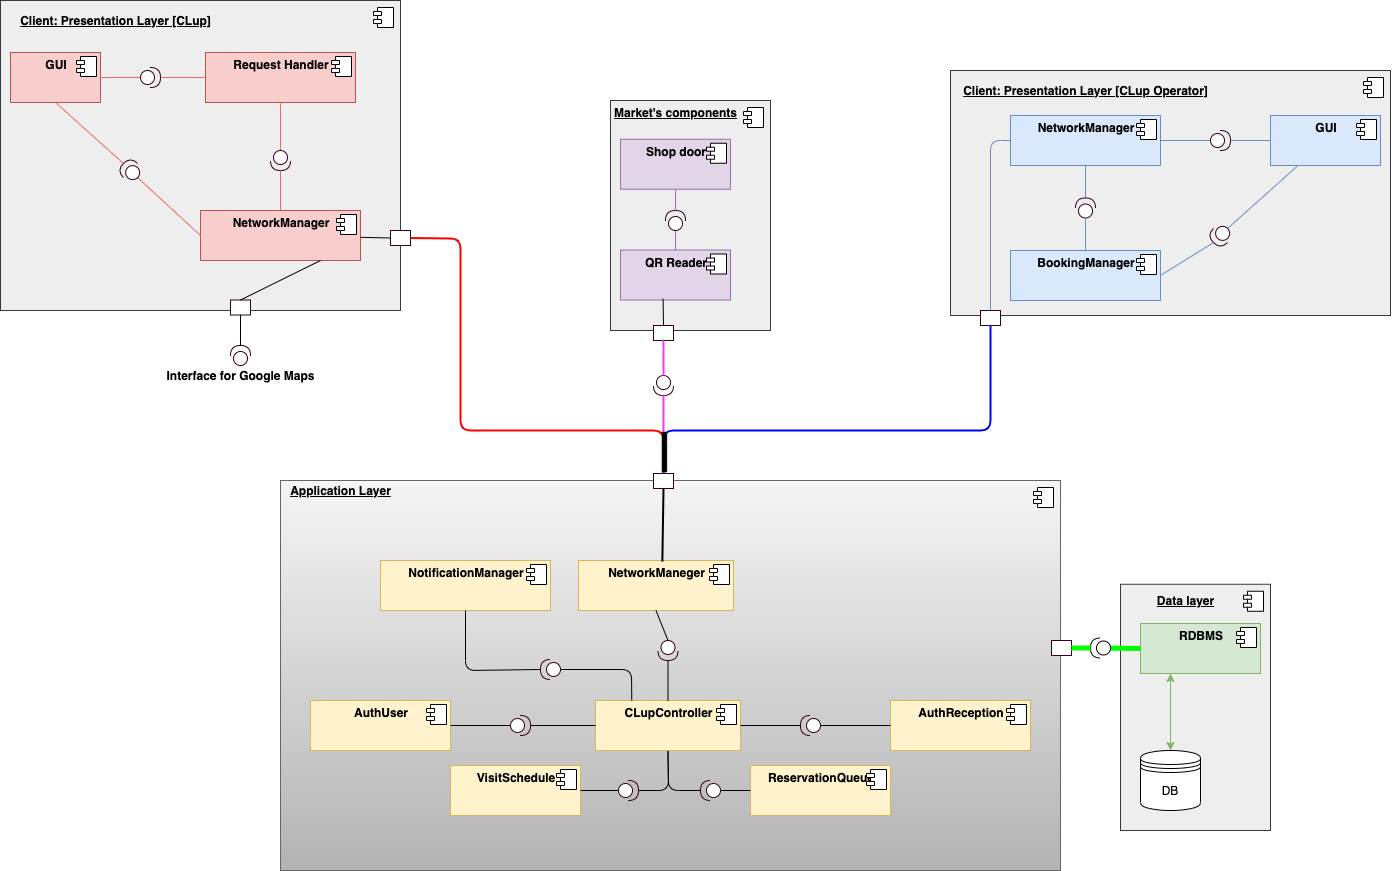
\includegraphics[scale=0.38]{diagrams/component_diagram.png}}
    \caption{Component Diagram}
\end{figure}



\subsection{Data Layer}

In our architecture the data layer is composed by a relational DB needed to store informations about users and their dynamics in the market. 

In particular it should be connected to the server placed in the application layer. To reach the goal we plan to adopt a \textbf{RDBMS} in order to deal with a relational database. Indeed, it ensures consistency of data due to the \textit{ACID} properties.

In addition, it can process a large amount of data, which is suitable for our application. 

Besides, due to a better efficiency, RDBMS provides \textit{horizontal fragmentation}. It allows to fragment entities of our model with respect to each different market. This is why tuples regarding different markets will never be queryied together. The only which won't be fragmented is the Market entity. 

Moreover, it includes a software program which is designed to capture request over a network of the application server. From this each user and receptionist in fact could retrieve informations needed through SQL Query by connecting to it.  


An other important aspect is the security of the data due to mitigate any risks of violation. In order to do that we limit its access exclusively only to the application server. Communication between them will be also encrypted and accounts' passwords will be hashed.




\section{Deployment view}


\begin{figure}[H]
  \label{fig:deployment}
  \centering
  \makebox[\linewidth]{
  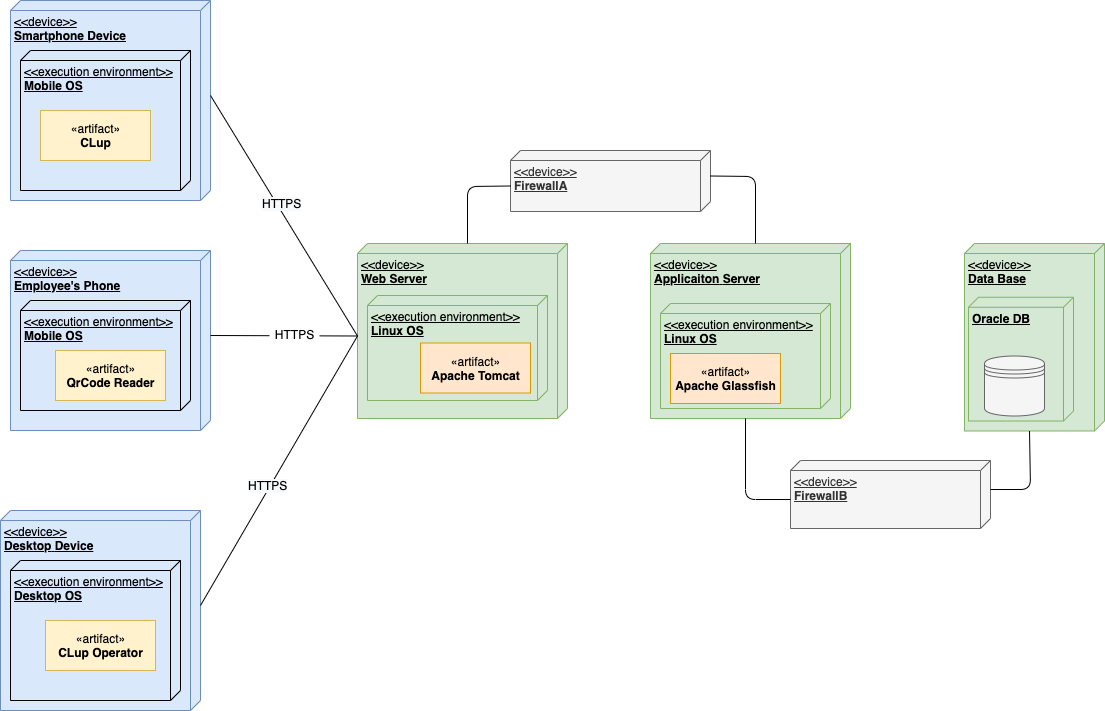
\includegraphics[scale=0.38]{diagrams/deployment.png}}
    \caption{Deployment Diagram}
\end{figure}



In this section we'll explain the structure of our run-time system and the interaction between the hardware and the software parts. This is shown in the deployment diagram in the figure~\ref{fig:deployment}. 

For the client's side, CLup and CLup Operator will be hosted respectevely on a mobile and desktop device. Softwares will be designed both following a cross-platform development. 
We choose cross-platform to ensure an easier and quicker implementation; moreover it includes a better uniformity and maintenability.   
The main OSs choosen are respectevely iOS and Android for CLup and macOS and Windows for CLup Operator.
In addition is provided a third device used by a generic employee of the market which, interfaced with a QRCode scanner, sends to the server any request for entering or leaving  the market.
Instead, the server is organized as well following a 3 Tier Server Architecture. Each tier is composed of:

\begin{enumerate}
\item \textbf{Web Server}: it's the node to which every clients connect. It handles each request from the clients connecting by HTTPS. It's built using \textbf{Apache Tomcat} %which can provide a web server. 
This, supported by Apache Software Foundation, a nonprofit corporation, is an open source software which is lightweight and suitable for our web server;
\item \textbf{Application Server}: this node hosts the core of our business logic. In particular we set \textbf{Apache Glassfish} which is leading of the Java EE standard to run servlets. Compared to Tomcat, is a full-blown Java EE application server, because it includes more features. Indeed it provides backup and recovery services due to a better availability a reliability;

\item \textbf{Data Base}: this machine contains each data of our system. In fact it's composed by a RDBMS in order to store and retrieve data. Besides, we choose \textbf{Oracle DB} from Oracle Corporation as management system on it. We choose it because of its high performances, which are necessary to process data quickly. In particular it can handles large volume of data since it have to manage a large number of users' requests simultaneously;
\end{enumerate}


Each tier is divided from the others with \textbf{2 Firewalls} which aim to filter any incoming and outgoing network traffic.
In particular:

\begin{itemize}

\item \textbf{FirewallA}: it filters traffic coming from the WS to AS. It allows requests from receptionist, logged user and employees' devices. This is due to mantaining the application server's integrity;

\item \textbf{FirewallB}: this protects the DB by filtering any packets, except for the application server. In this way we gurantee an high security against any data violation; 
\end{itemize}




\section{Runtime view}




\begin{figure}[H]
  \label{ReservatioSD}
  \centering
  \makebox[\linewidth]{
  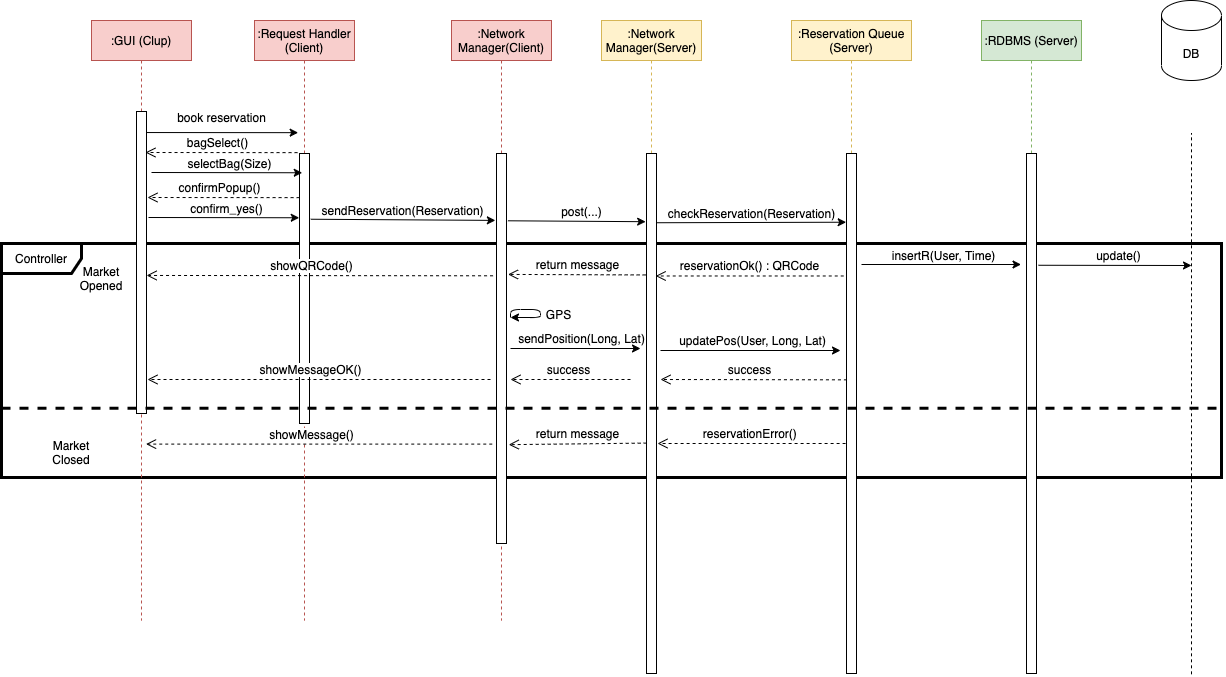
\includegraphics[scale=0.52]{diagrams/ReservationSD.png}}
    \caption{}
\end{figure} 


\begin{figure}[H]
  \label{VisitSD}
  \centering
  \makebox[\linewidth]{
  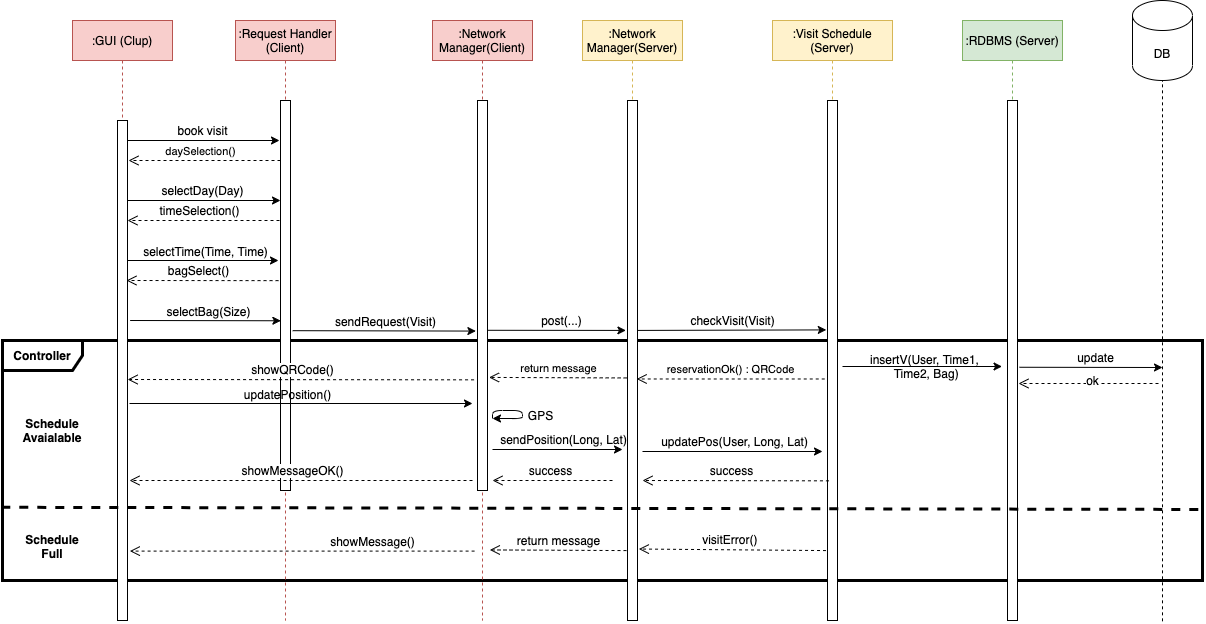
\includegraphics[scale=0.52]{diagrams/VisitSD.png}}
    \caption{}
\end{figure} 


\begin{figure}[H]
  \label{EntryExitSD}
  \centering
  \makebox[\linewidth]{
  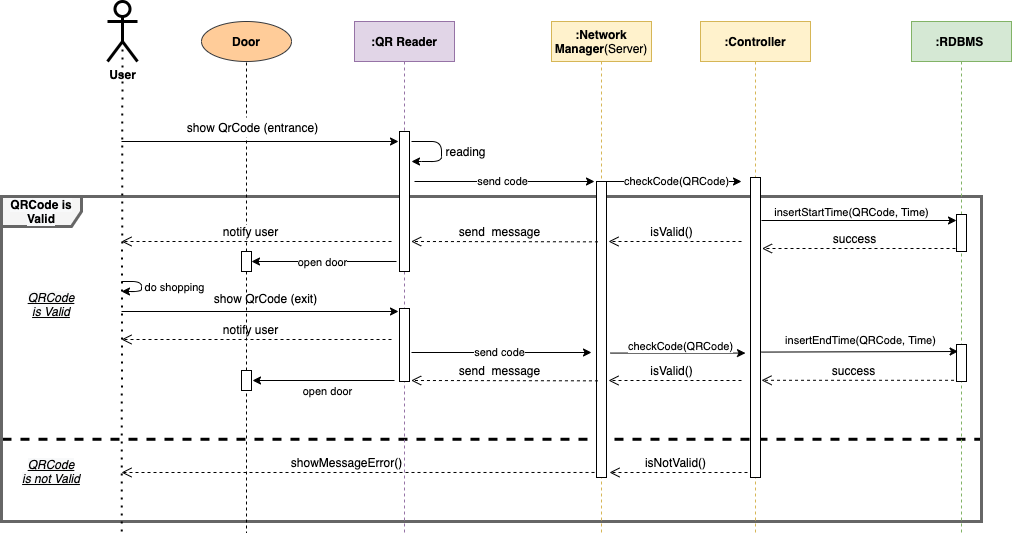
\includegraphics[scale=0.52]{diagrams/EntryExitSD.png}}
    \caption{}
\end{figure} 


\begin{figure}[H]
  \label{PostponeReservationSD}
  \centering
  \makebox[\linewidth]{
  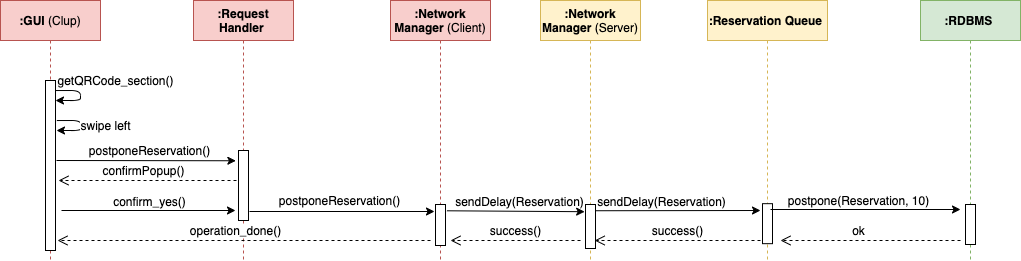
\includegraphics[scale=0.52]{diagrams/PostponeReservationSD.png}}
    \caption{}
\end{figure} 


\begin{figure}[H]
  \label{DeleteVisitSD}
  \centering
  \makebox[\linewidth]{
  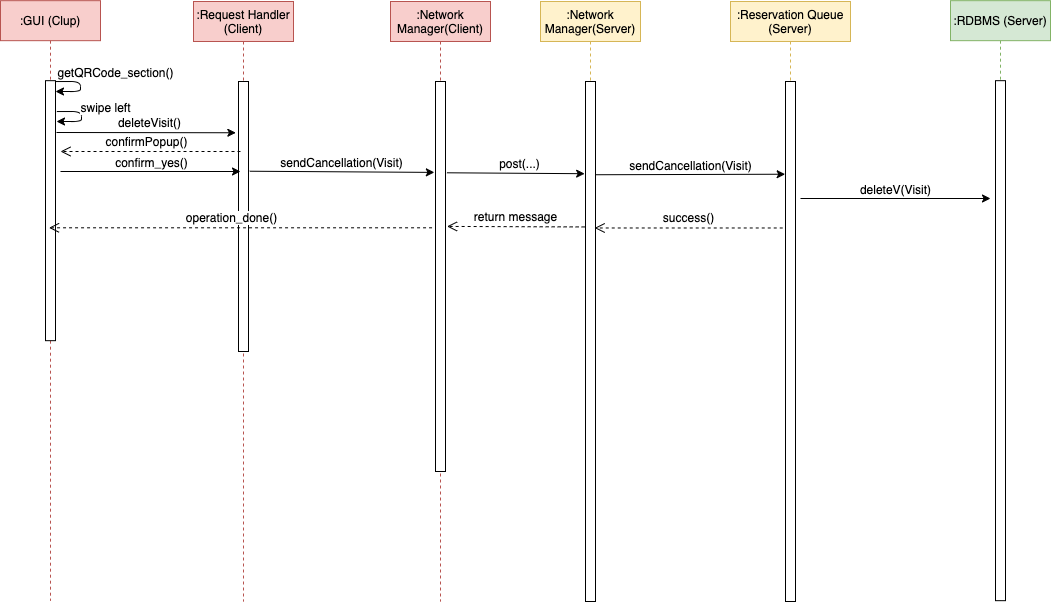
\includegraphics[scale=0.52]{diagrams/DeleteVisitSD.png}}
    \caption{}
\end{figure} 

\begin{figure}[H]
  \label{MobileUserSD}
  \centering
  \makebox[\linewidth]{
  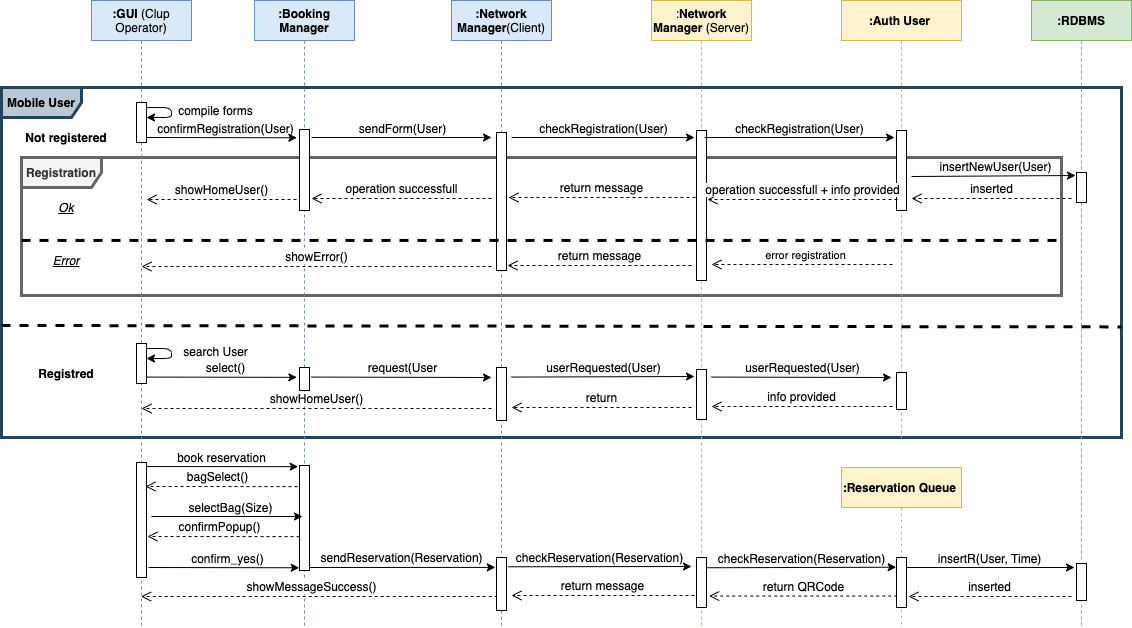
\includegraphics[scale=0.52]{diagrams/MobileUserSD.png}}
    \caption{}
\end{figure} 


\begin{figure}[H]
  \label{NotificationsSD}
  \centering
  \makebox[\linewidth]{
  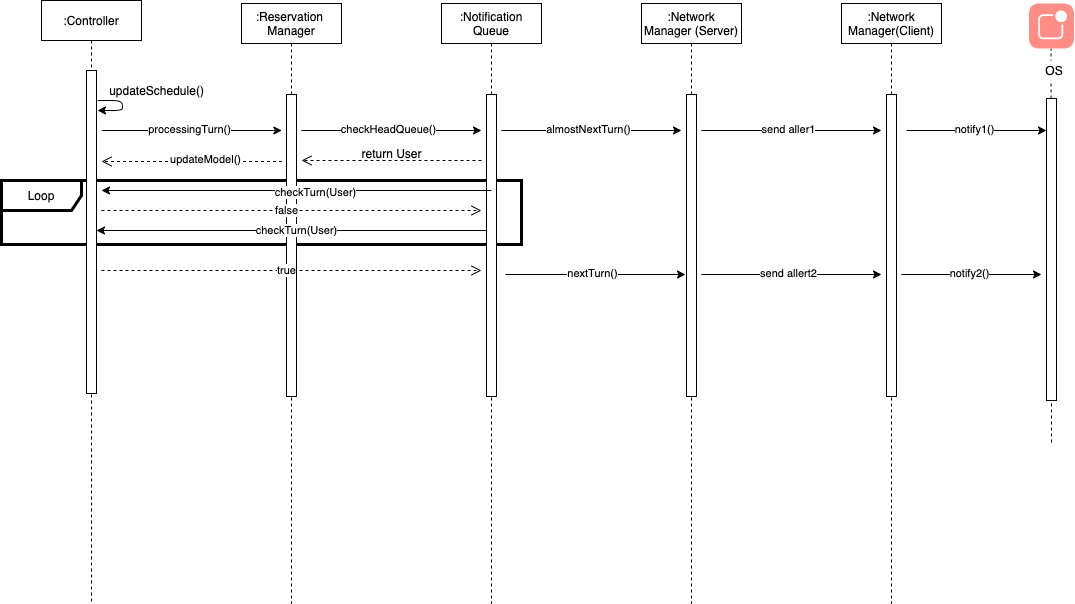
\includegraphics[scale=0.52]{diagrams/NotificationsSD.png}}
    \caption{}
\end{figure} 








\section{Component interfaces}
ogni componente
app
server+db
laptop receptionist

\section{Selected architectural styles and patterns}
mvc + tier + ..

\section{Other design decisions}

security+google api
asyncrnous coomunication because eccc
